\clearpage
\newpage
\section*{Extended Data}
\pagebreak

\renewcommand{\figurename}{Extended Data Fig.}
\renewcommand{\tablename}{Extended Data Table}
% \renewcommand{\thetable}{S\arabic{table}}
\setcounter{figure}{0}

\begin{figure}[t]
\centering
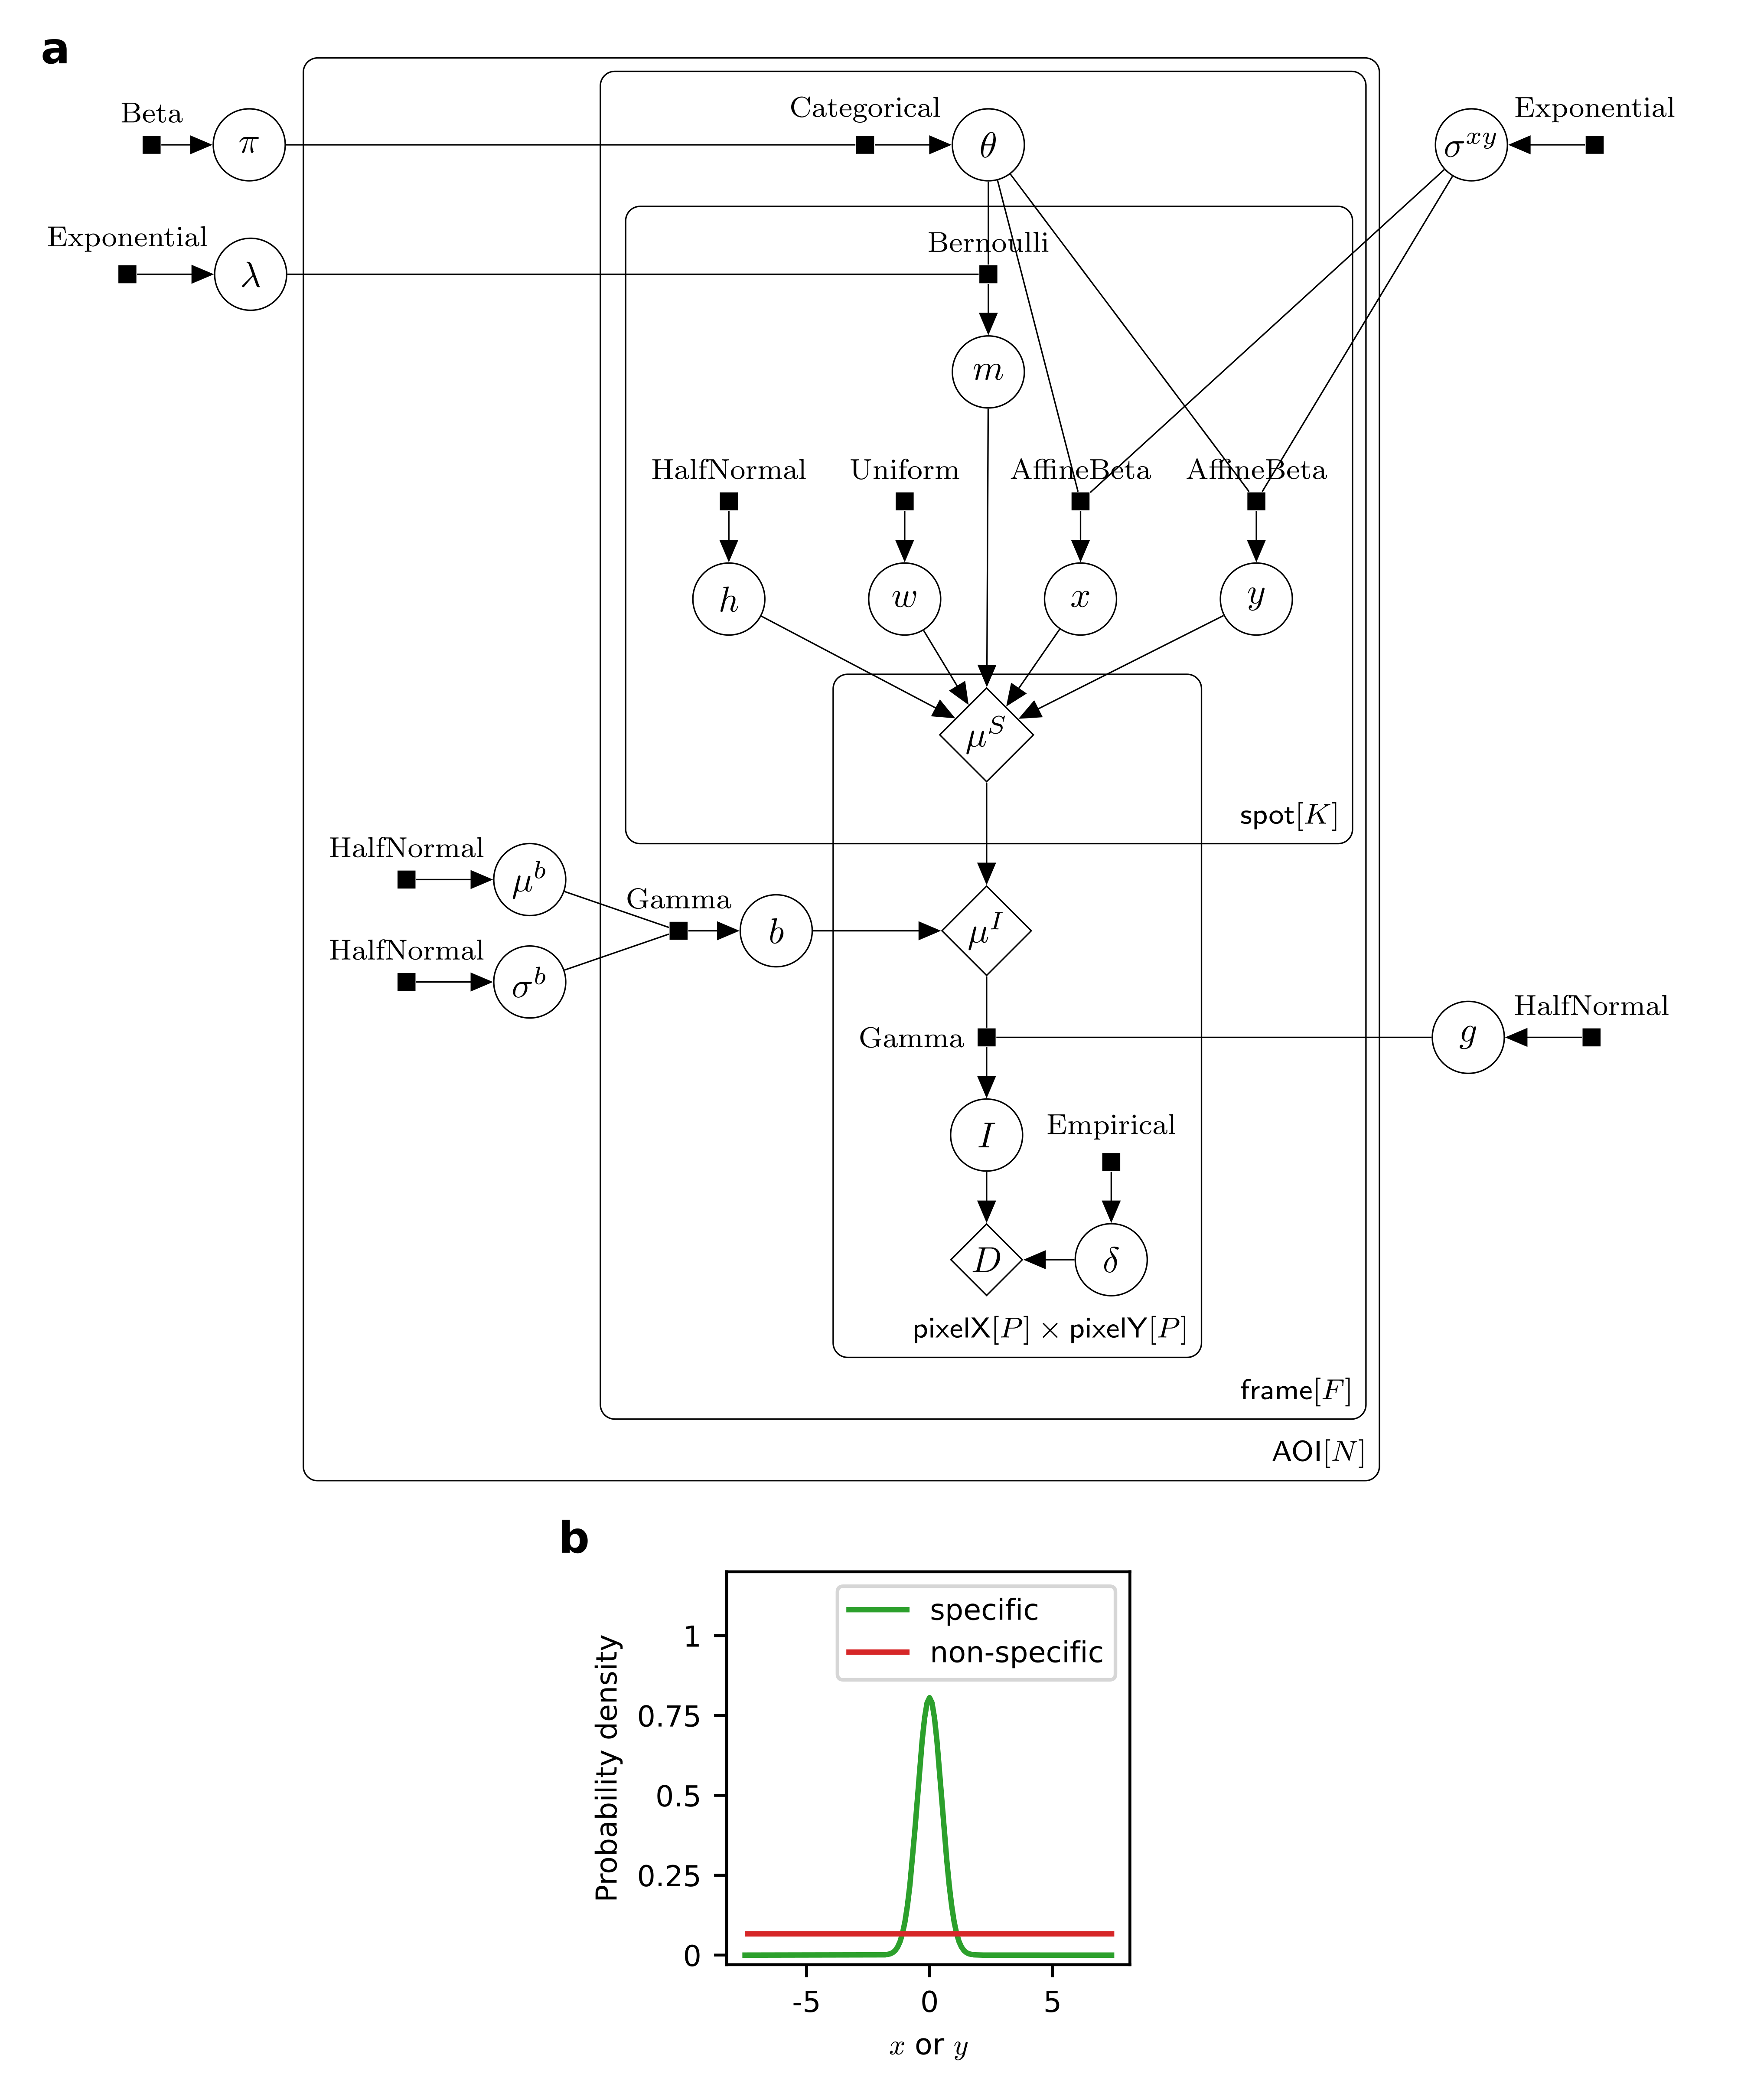
\includegraphics[width=\textwidth]{extended-data/figure1/figure1.png}
\label{fig:full_model}
\end{figure}

%\addtocounter{figure}{-1}
\begin{figure} [t]
\caption{\textbf{Extended graphical representation of the generative probabilistic model and the prior distributions for $x$ and $y$ spot position parameters.} \textbf{a}, Directed factor graph representation \cite{Bishop2006-oa} of model parameters and parameter distributions. Model parameters are depicted as circles, parameter distributions as small filled squares, and deterministic functions as diamonds. Names of the probability distributions are written next to the squares. Input parameters and output parameters are connected by lines, with an arrow pointing towards the dependent parameter. Observed image ($D$) is the sum of the noisy photon-dependent image ($I$) and the photon-independent camera offset ($\delta$). Plates (rounded rectangles) contain nodes that are repeated for the number of instances displayed at the bottom-right corner: number of AOIs ($N$), frame count ($F$), maximum number of spots in a single image ($K$), and number of image pixels ($P \times P$). \textbf{b}, Prior distributions of $x$ and $y$ for specific and non-specific binding. Probability densities for $x$ and $y$ are defined in the range $\left[ -(P+1)/2, (P+1)/2 \right] $ relative to the target molecule and are conditional on the identity of the spot (specific or non-specific).  Probability densities for $x$ and $y$ parameters are identical. }
\end{figure}
\clearpage

\begin{figure}[h]
\centering
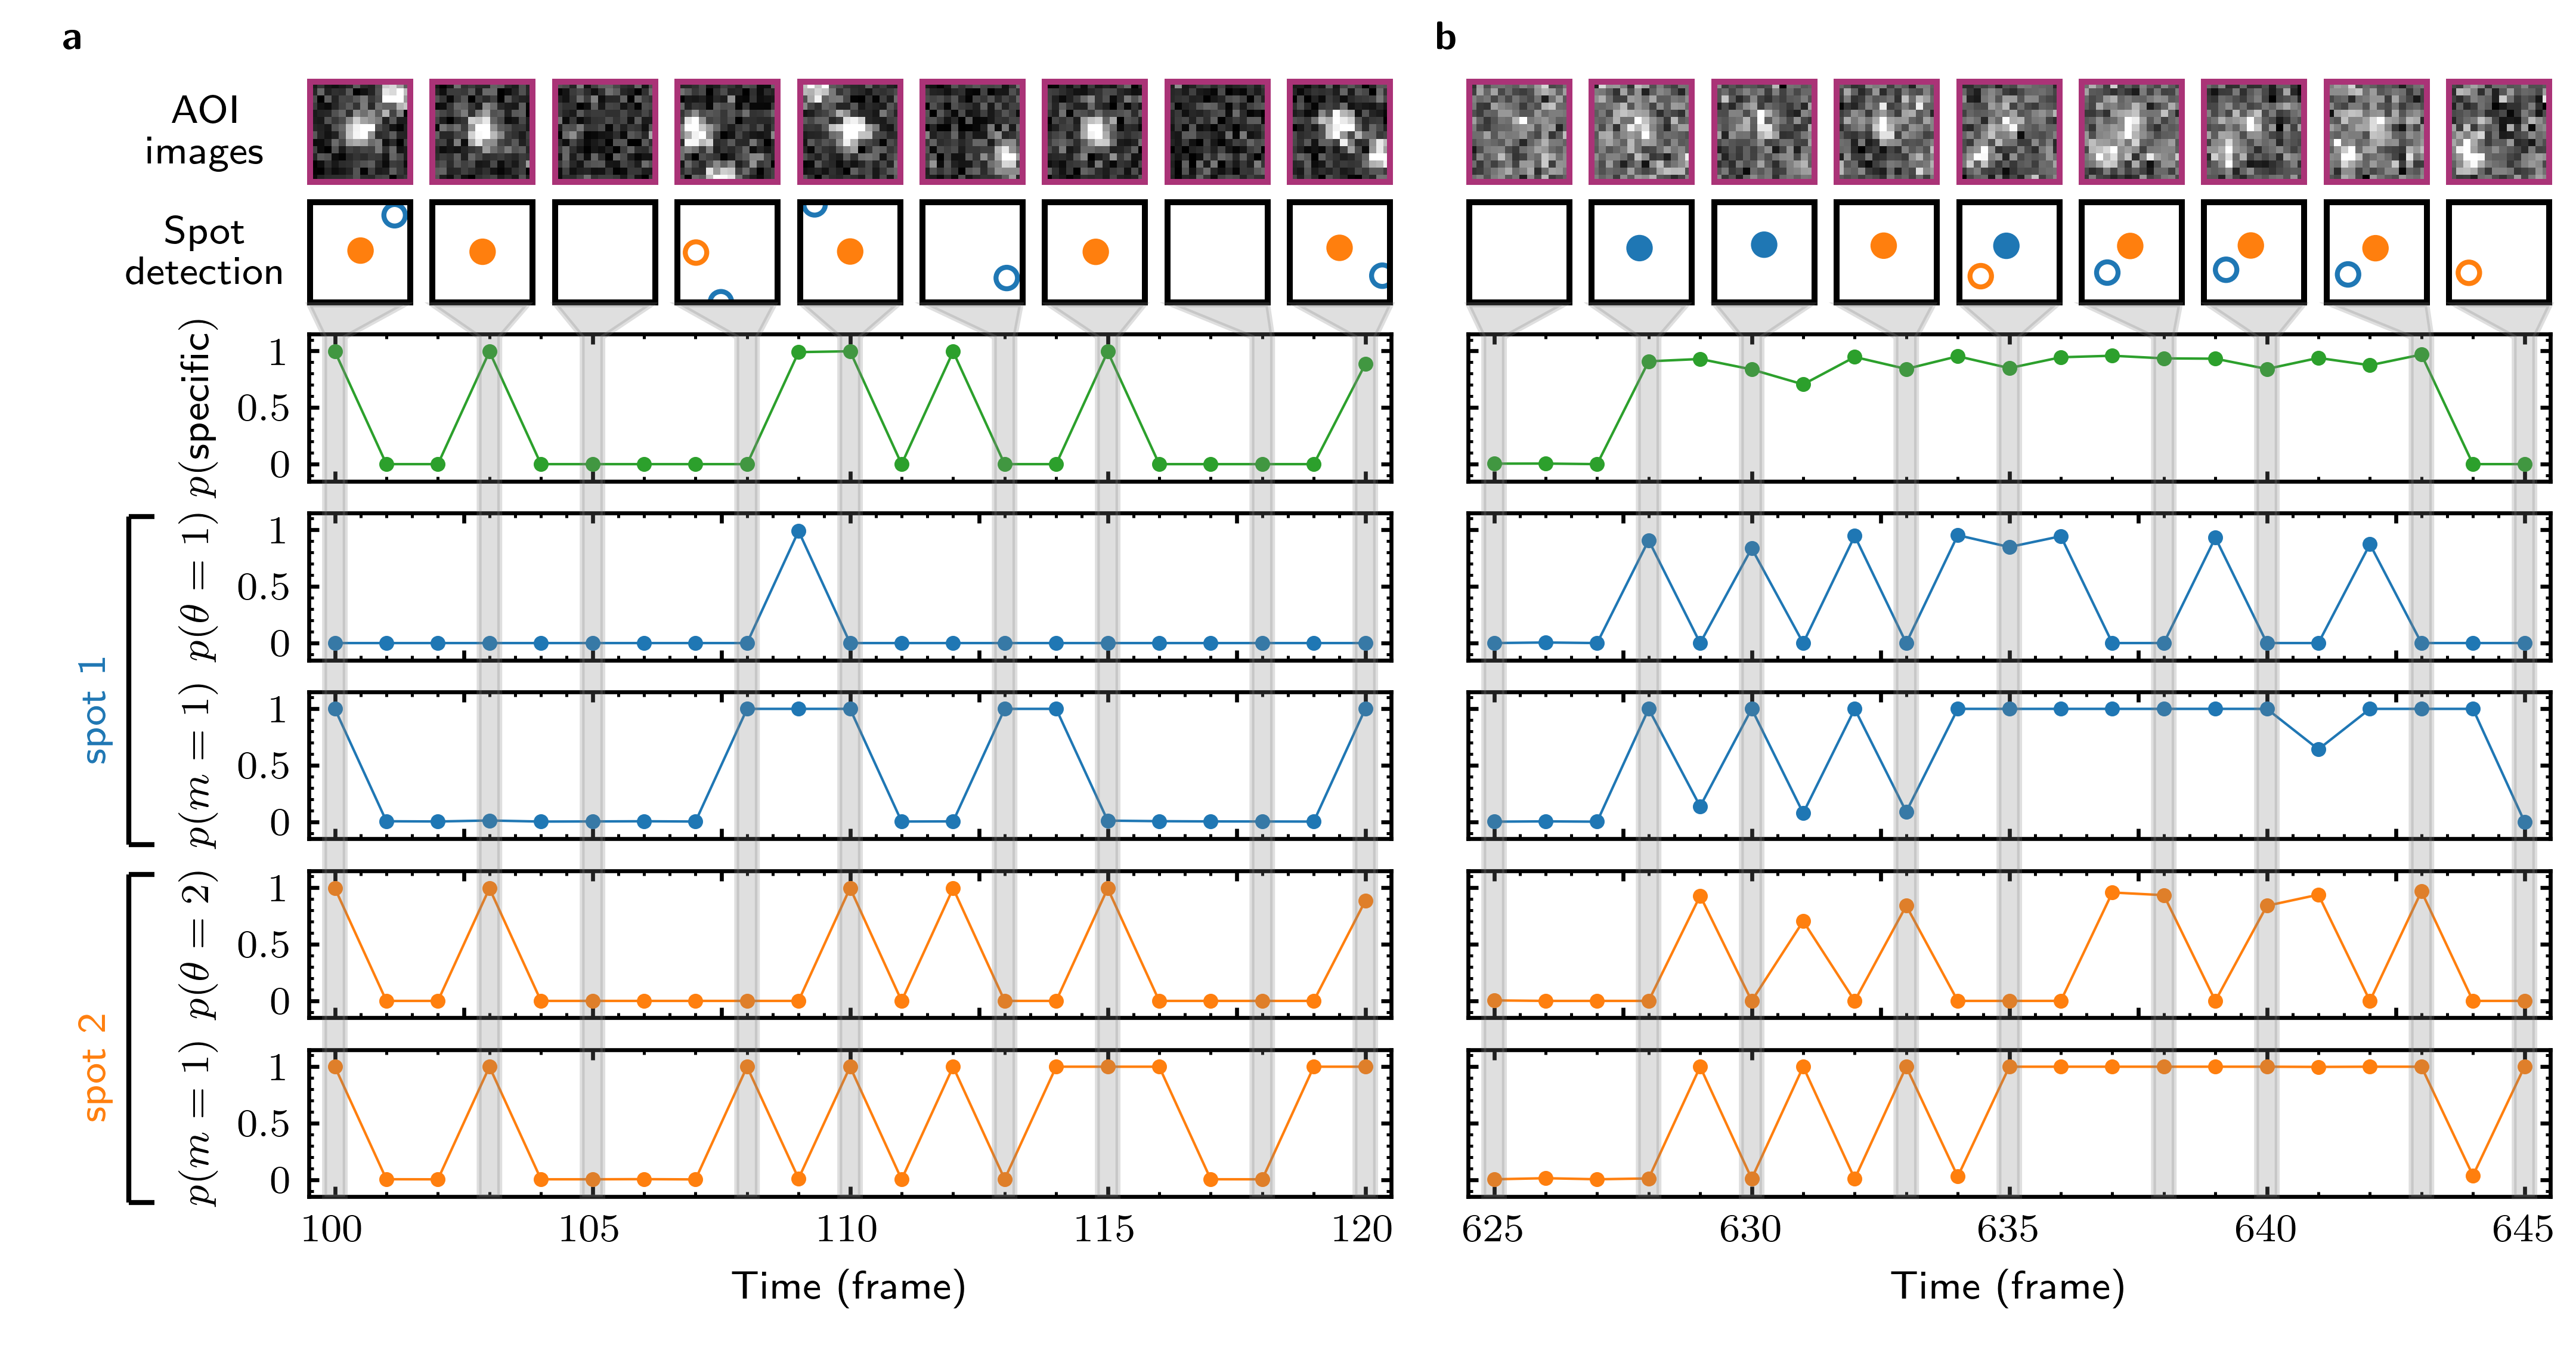
\includegraphics[width=\textwidth]{extended-data/figure2.png}
\caption{\textbf{Tapqir analysis and inferred spot probabilities.} The first two rows and $p(\mathsf{specific})$ graph are as in Fig. 3. The new graphs show the probability of a spot being target-specific ($p(\theta=k)$ for  $k^\mathrm{th}$ spot) and the probability of spot presence ($p(m=1)$) of spot 1 (blue) and spot 2 (orange).  }
\end{figure}
\pagebreak

% extended figure 3
\begin{figure}[h]
\centering
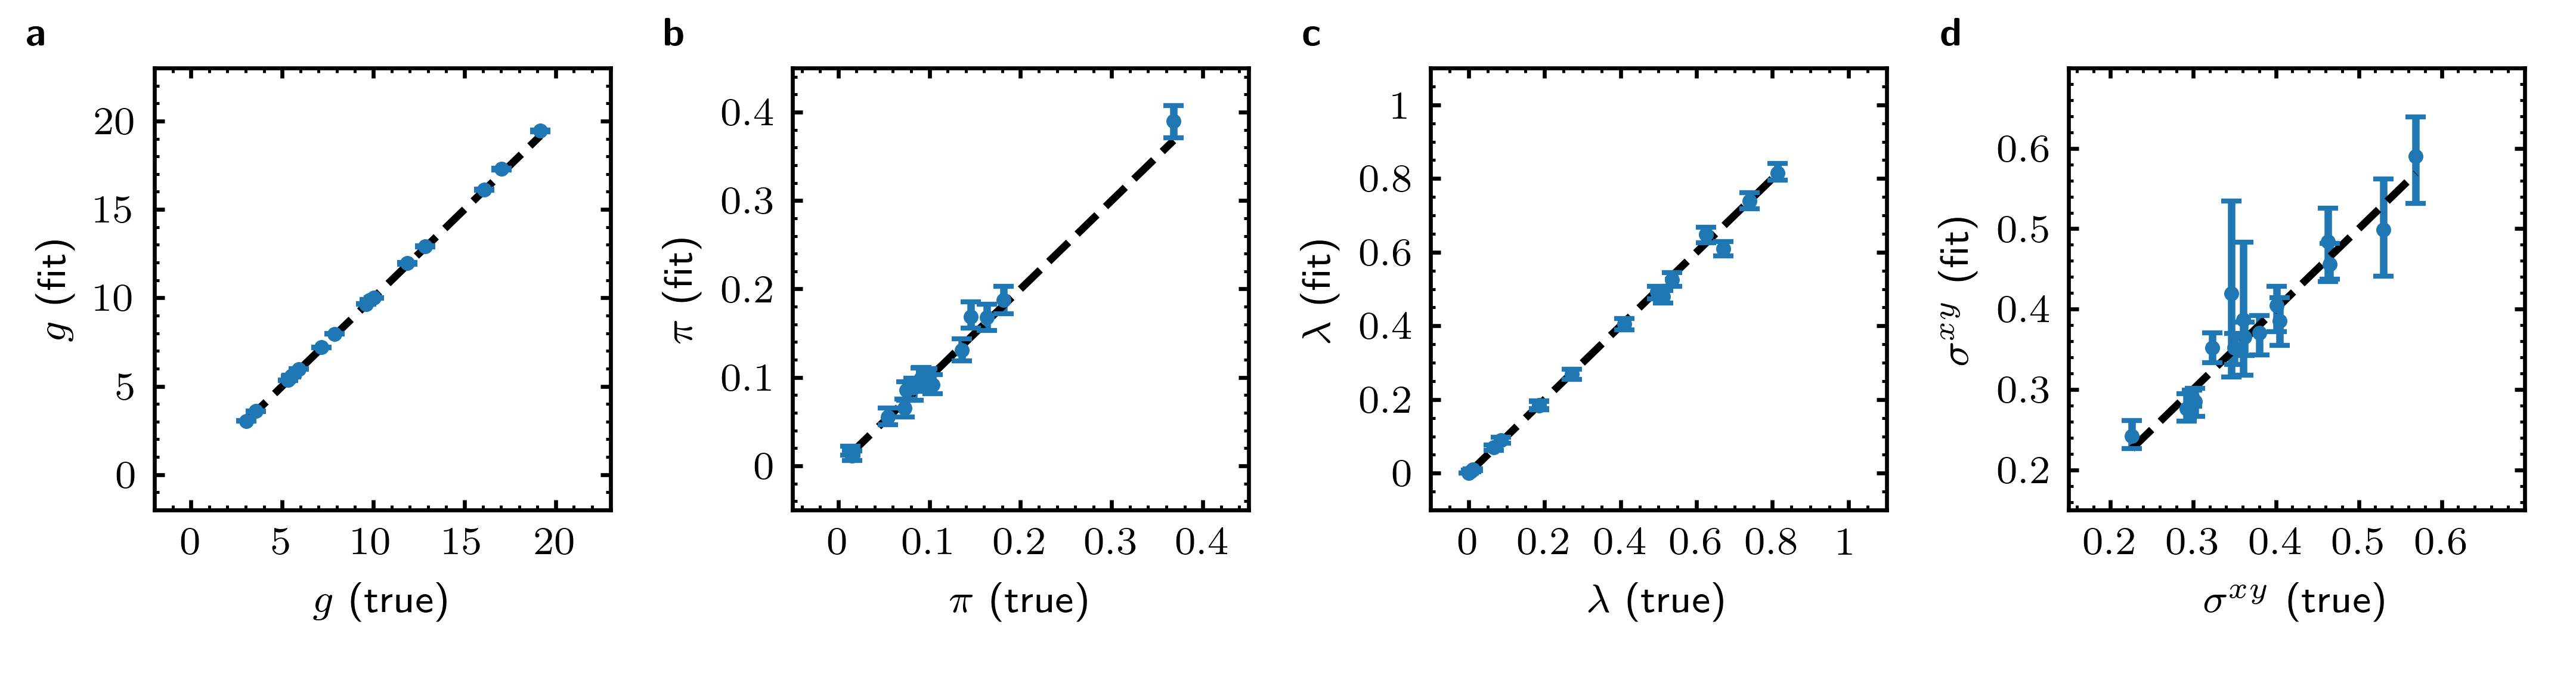
\includegraphics[width=\textwidth]{extended-data/figure3.png}
\caption{\textbf{Tapqir analysis of image data simulated using a broad range of global parameters.} Simulations (see Methods) consist of 16 datasets where values of global parameters ($\pi$, $\lambda$, $\sigma^{xy}$, and $g$) where randomly generated for each dataset (Supplementary Data 2). Simulated data were fit with Tapqir, and parameter values from the fit (with 95\% CI) are plotted against the true parameter values. To guide the eye, dashed lines  indicate identical true and fit values. \textbf{a}, Average specific binding probability $\pi$. \textbf{b}, Nonspecific binding rate $\lambda$. \textbf{c}, Proximity parameter $\sigma^{xy}$. \textbf{d}, Gain of the camera $g$. }
\label{fig:tapqir_global}
\end{figure}
\pagebreak

% extended figure 4
\begin{figure}[t]
\centering
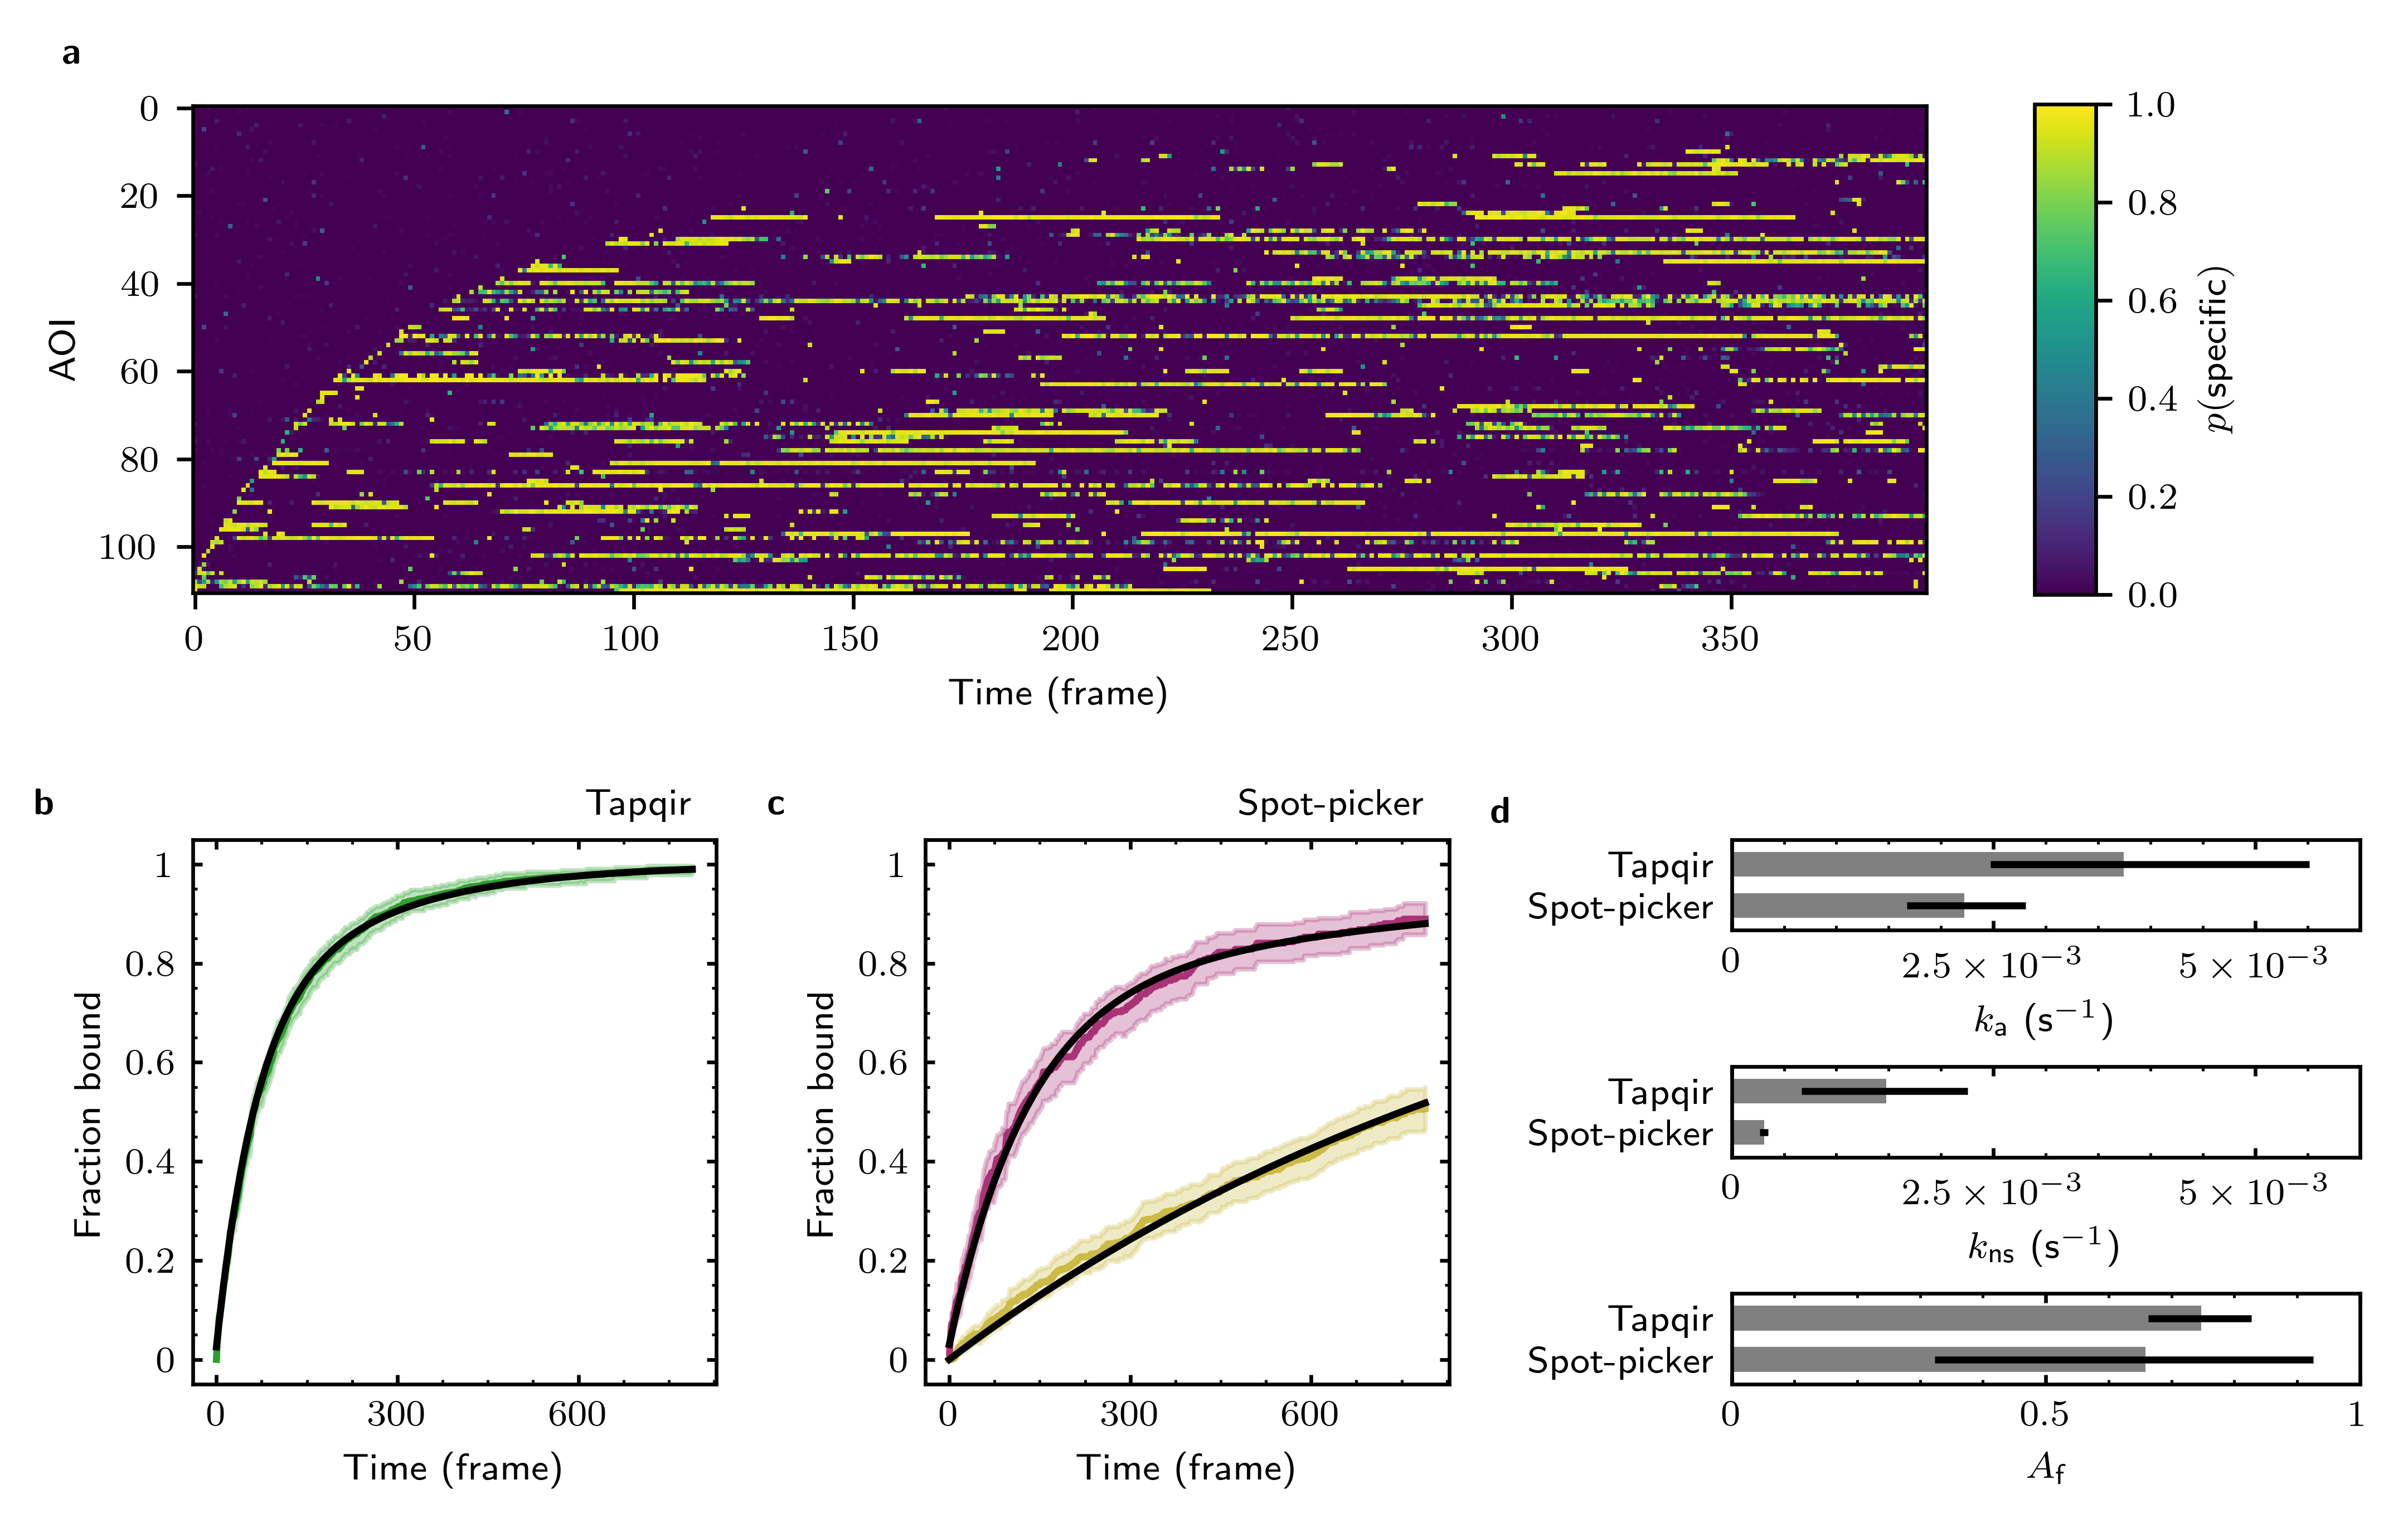
\includegraphics[width=\textwidth]{extended-data/figure4.png}
\caption{\textbf{Additional example showing extraction of target-binder association kinetics from experimental data.} Data are from Data set A (see Extended Data Table 1).  Results are plotted as in Fig. 7, except that for clarity only every $2^\mathrm{nd}$ frame and every $3^\mathrm{rd}$ AOI is shown in \textbf{a}.}
\label{fig:rpb1snap549}
\end{figure}
\pagebreak

% extended figure 5
\begin{figure}[t]
\centering
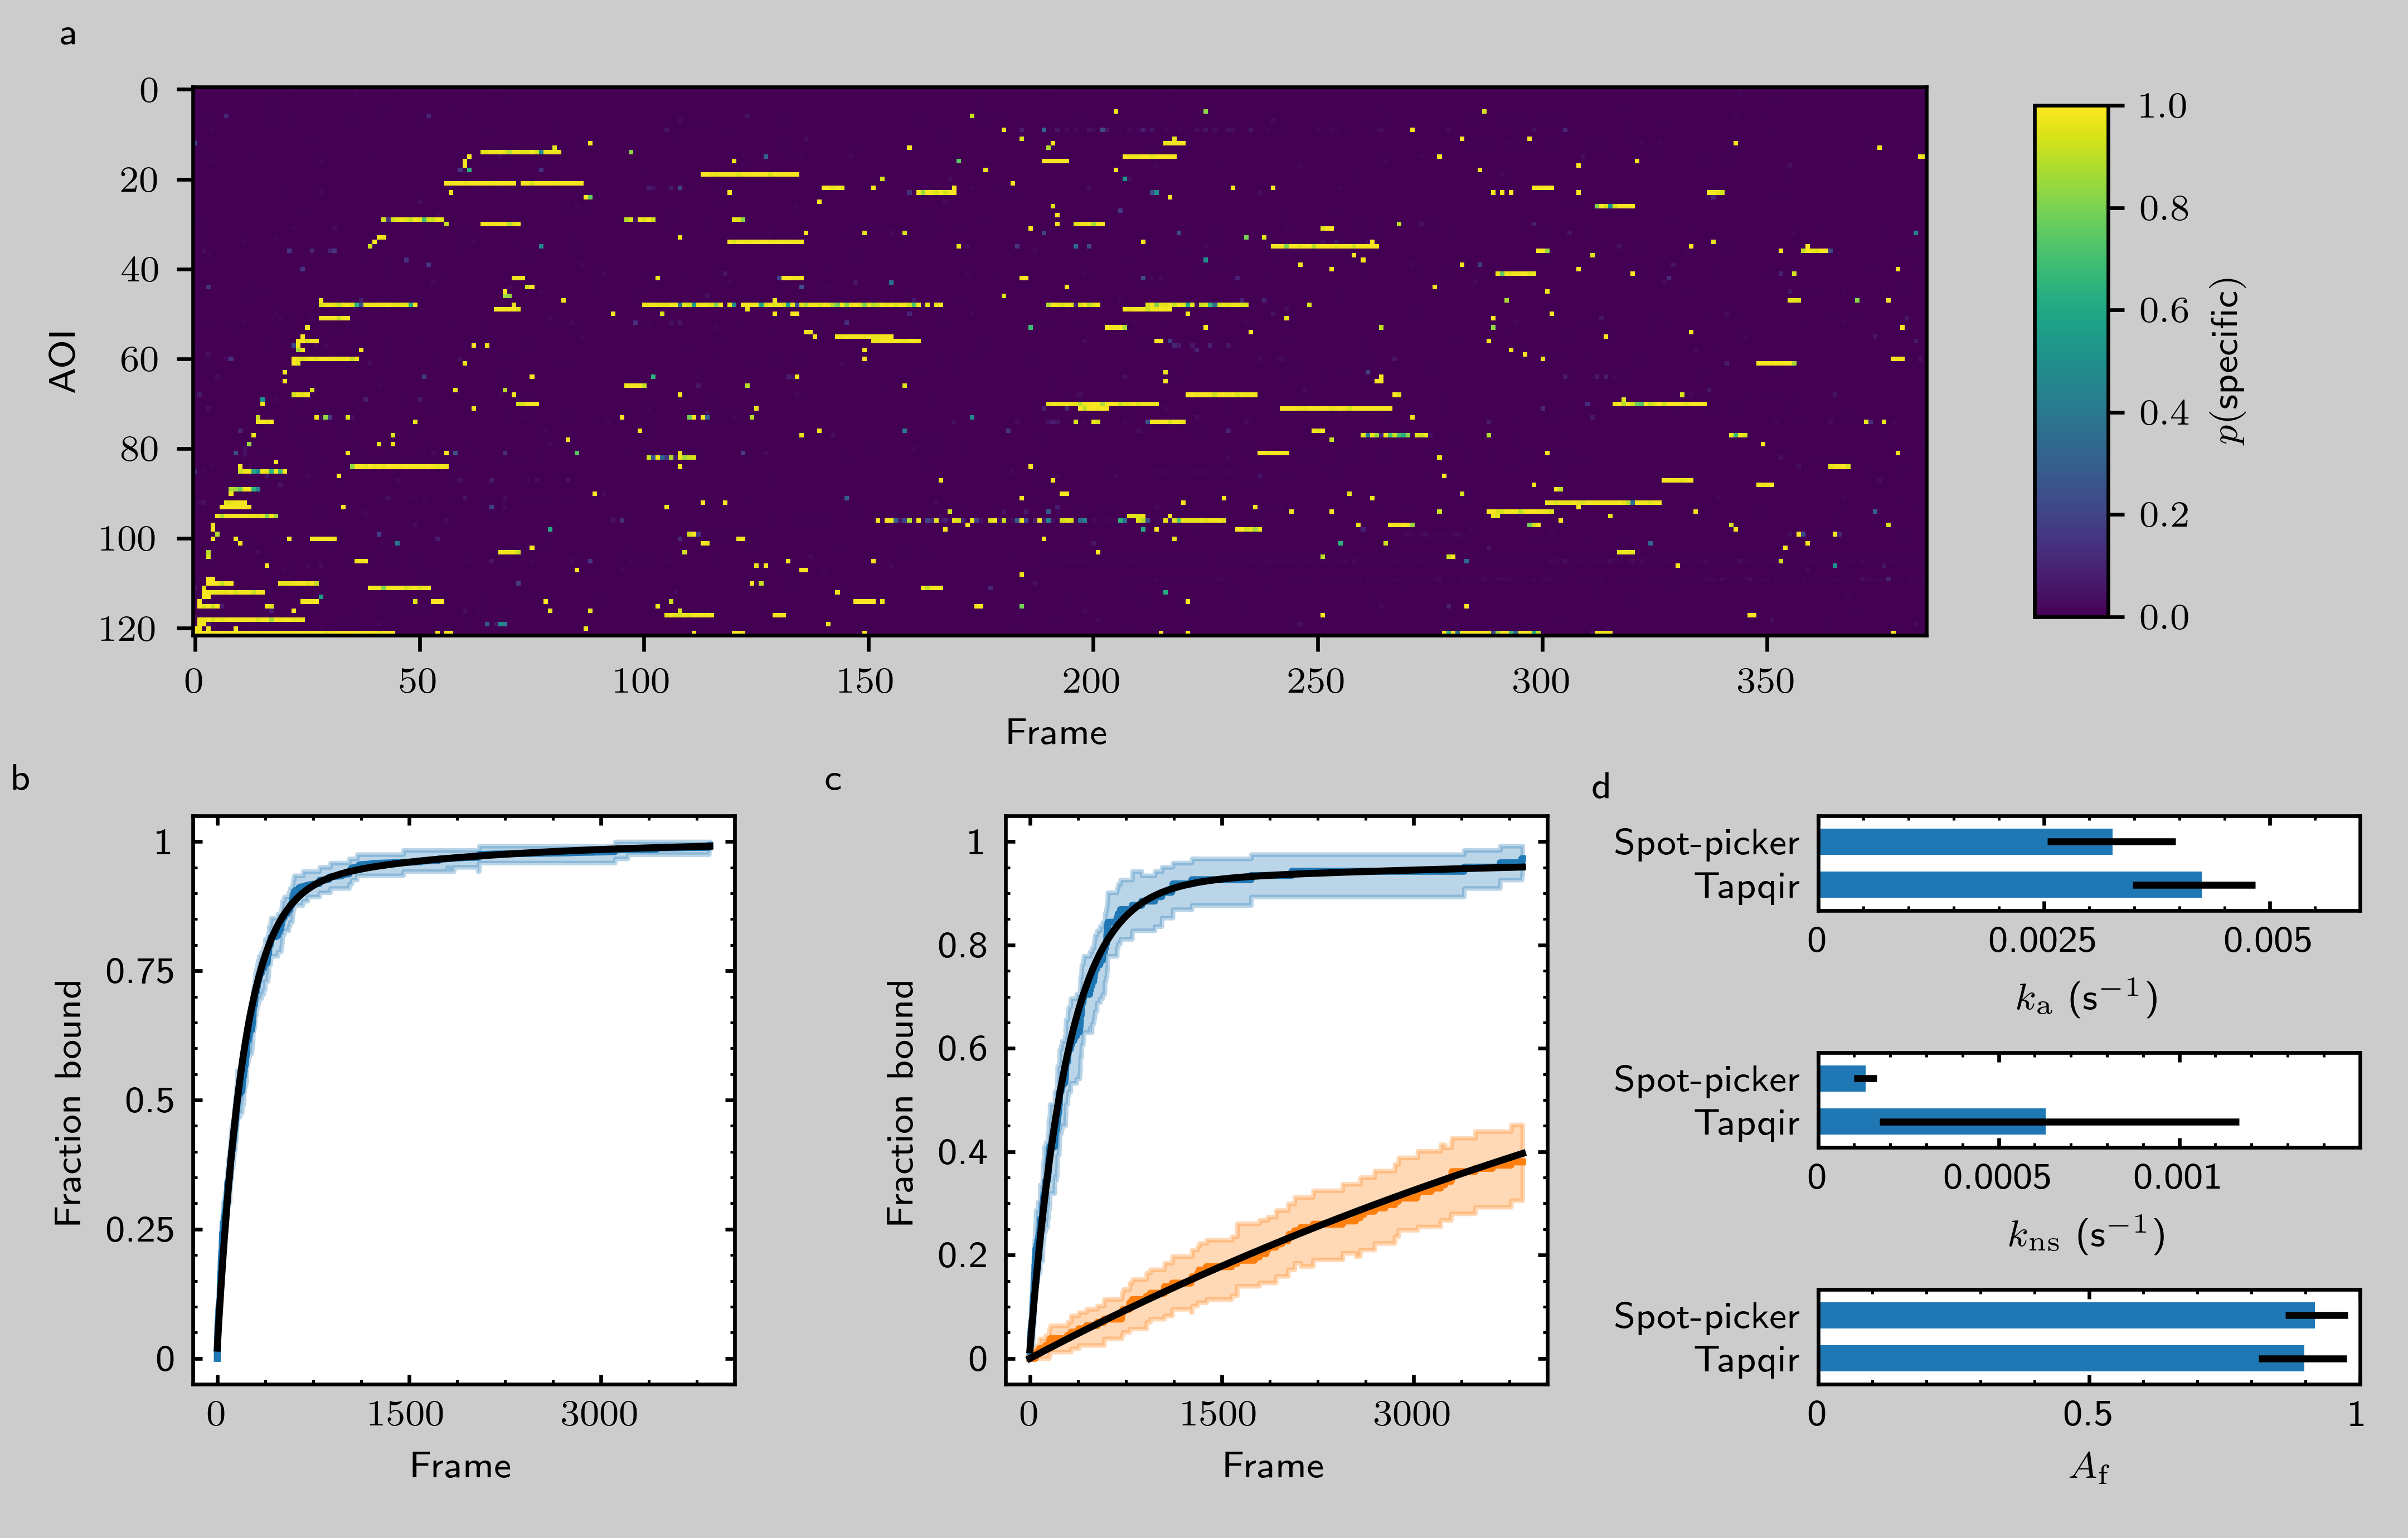
\includegraphics[width=\textwidth]{extended-data/figure5.png}
\caption{\textbf{Additional example showing extraction of target-binder association kinetics from experimental data.} Data are from Data set C (see Extended Data Table 1).  Results are plotted as in Fig. 7, except that for clarity only every $10^\mathrm{th}$ AOI is shown in \textbf{a}.}
\label{fig:sigma54_298P2993}
\end{figure}
\clearpage
\pagebreak


% extended figure 6
\begin{figure}[t]
\centering
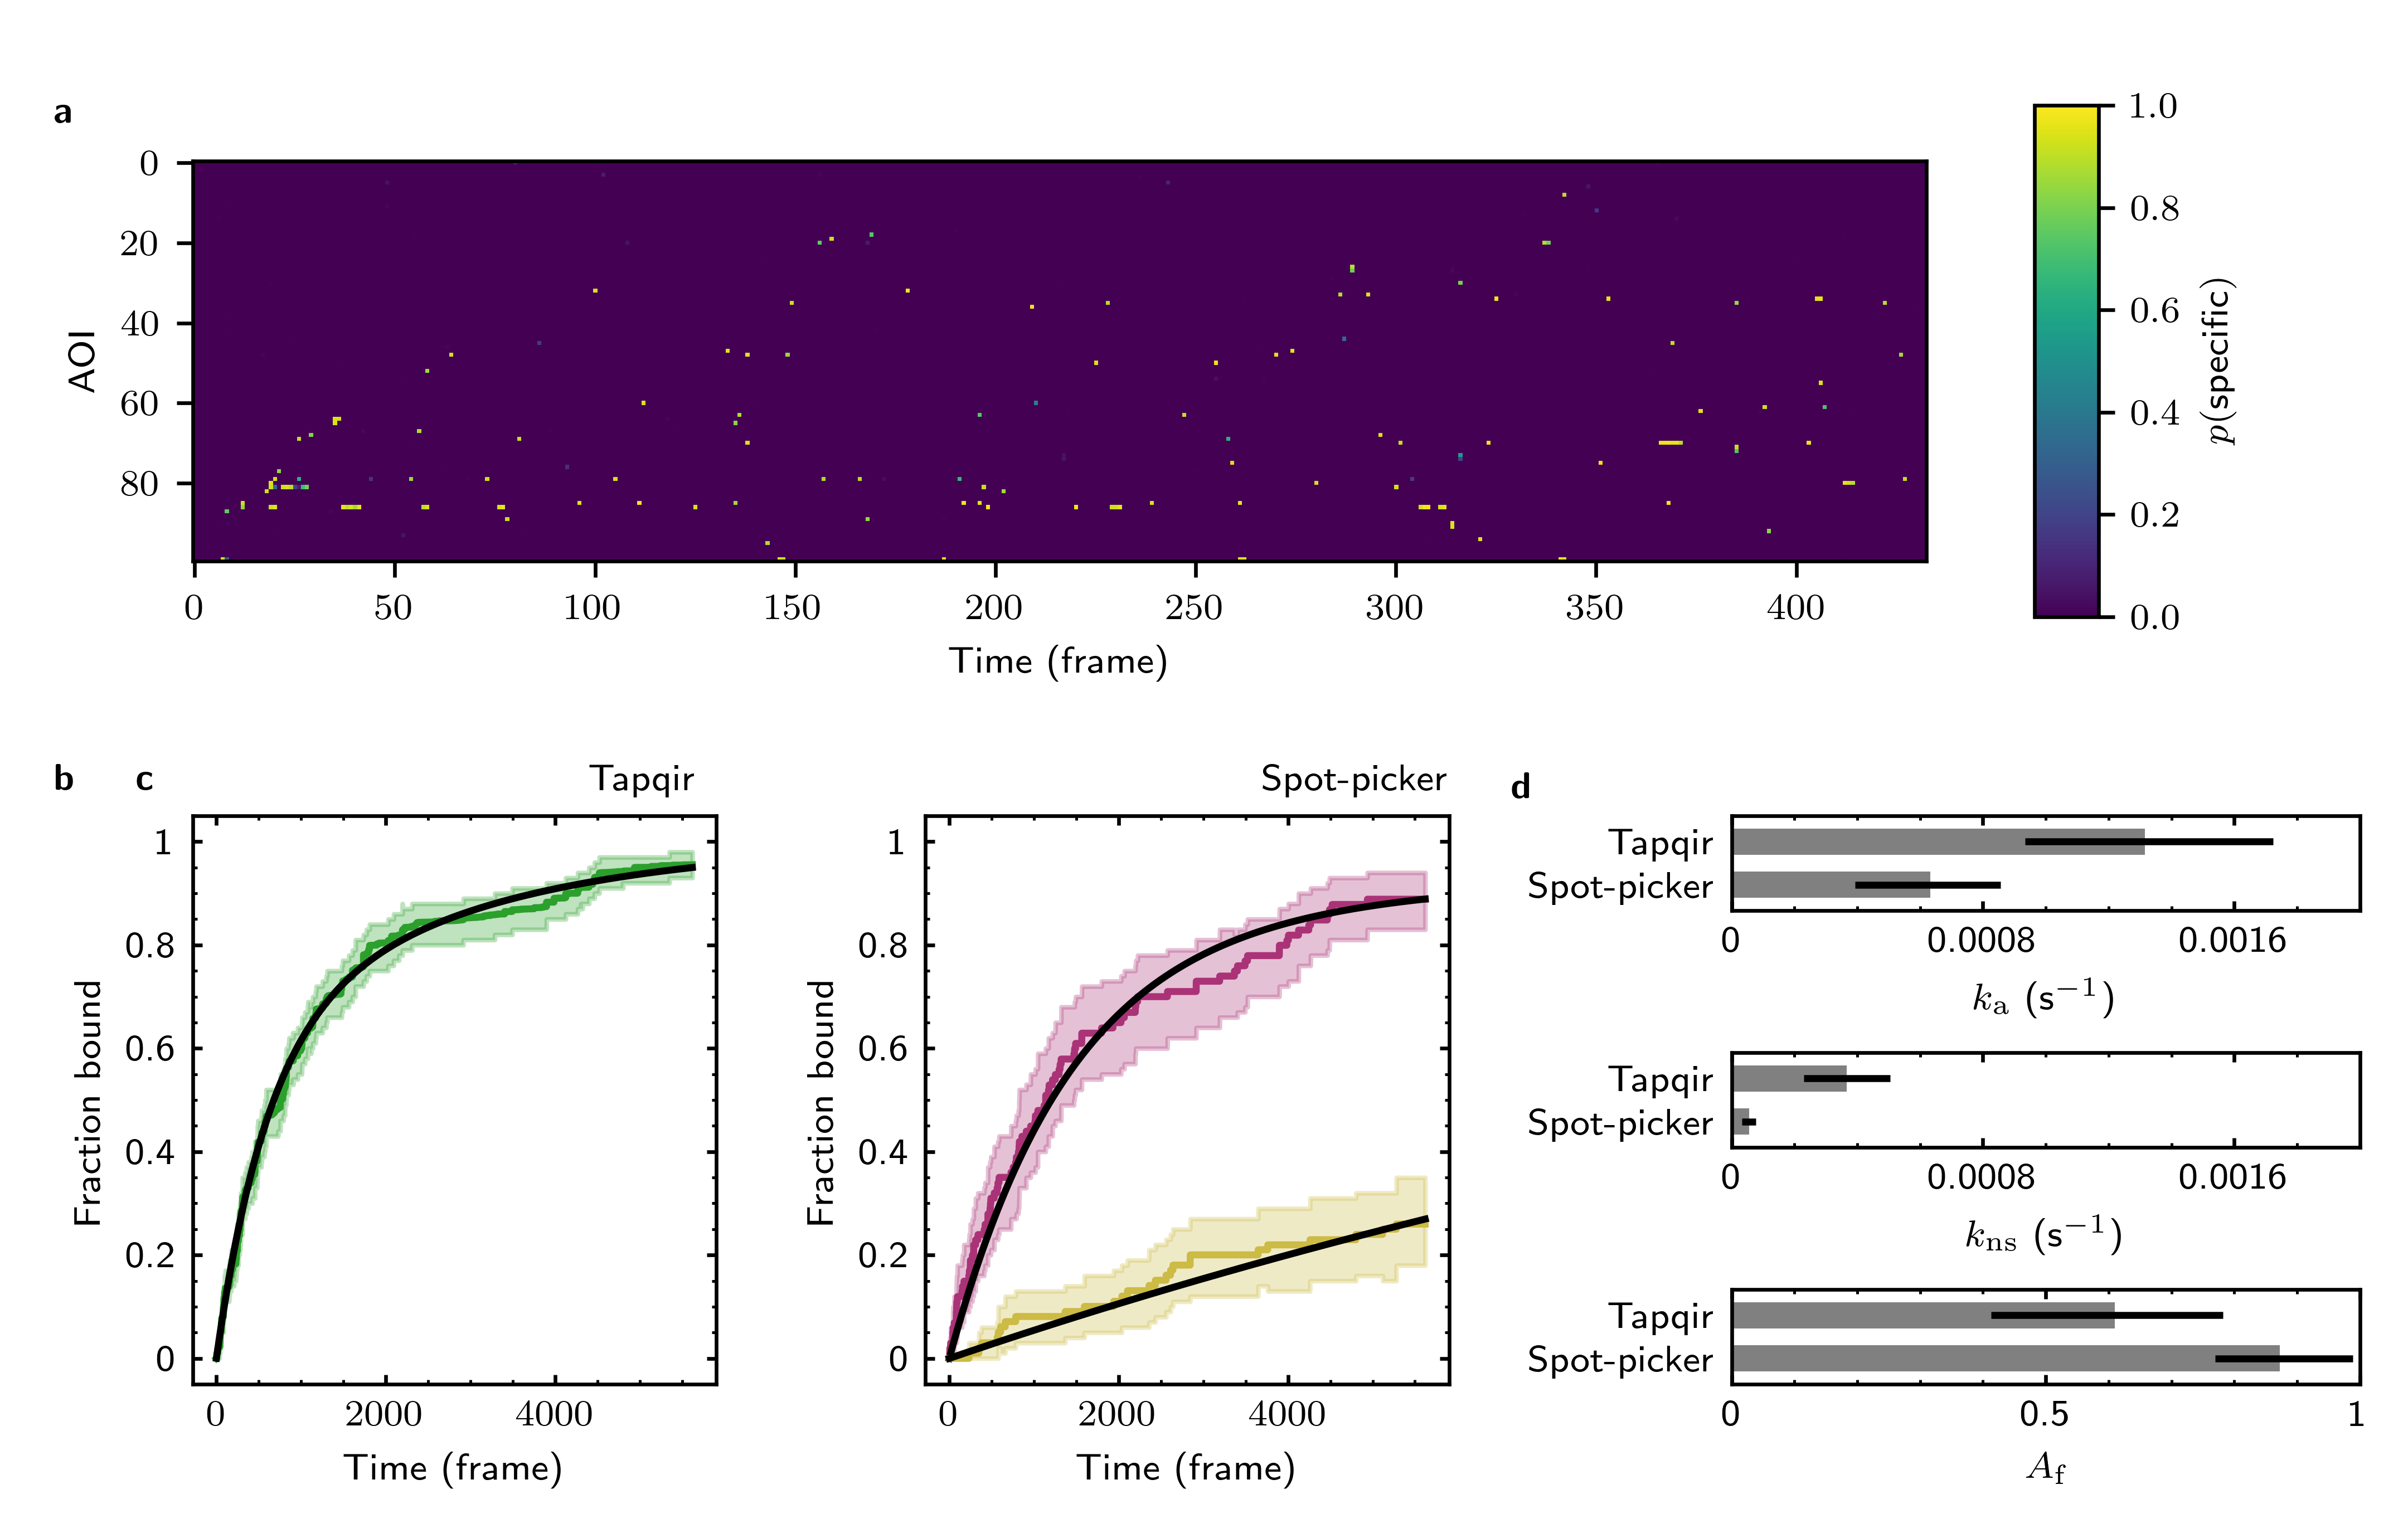
\includegraphics[width=\textwidth]{extended-data/figure6.png}
\caption{\textbf{Additional example showing extraction of target-binder association kinetics from experimental data.} Data are from Data set D (see Extended Data Table 1).  Results are plotted as in Fig. 7, except that for clarity only every $13^\mathrm{th}$ AOI is shown in \textbf{a}.}
\label{fig:greb}
\end{figure}
\clearpage
\pagebreak

\begin{table}[h]
\caption{\label{tab:datasets} \textbf{Experimental data sets.}}
\resizebox{\textwidth}{!}{%
% Use "S" column identifier to align on decimal point 
\begin{tabular}{ccccccc}
\toprule
Data set size\textsuperscript{a} & SNR & $\pi \: [95\% \: \mathrm{CI}]$ & $\lambda \: [95\% \: \mathrm{CI}]$ & $g \: [95\% \: \mathrm{CI}]$ & $\sigma^{xy} \: [95\% \: \mathrm{CI}]$ & Compute time\textsuperscript{b} \\
\midrule
\multicolumn{7}{l}{\parbox{1.2\textwidth}{Data set A: Binder, SNAP\textsubscript{f}-tagged \textit{S. cerevisiae} RNA polymerase II labeled with DY549; Target, transcription template DNA containing $5 \times$ Gal4 upstream activating sequences and \textit{CYC1} core promoter; Conditions, yeast nuclear extract supplemented with Gal4-VP16 activator and NTPs. From \cite{Rosen2020-zn}.}} \\
\\
\begin{tabular}[x]{@{}c@{}}$N = 331$, $F = 790$\\$N_c = 526$, $F_c = 790$\end{tabular} & $1.63$ &
$0.1022\:[0.1009, 0.1035]$ & $0.2958\:[0.294, 0.2970]$ & $6.507\:[6.505, 6.509]$ & $0.554\:[0.549, 0.557]$ & 6 h \\
\midrule
\multicolumn{7}{l}{\parbox{1.2\textwidth}{Data set B: Binder, 0.1 nM \textit{E. coli} $\sigma^{54}$ RNA polymerase labeled with Cy3; Target, 852 bp DNA containing the \textit{glnALG} promoter; Conditions, phyiological buffer, no NTPs. From  (Fig. 1E) of \cite{Friedman2013-sf}.}} \\
\\
\begin{tabular}[x]{@{}c@{}}$N = 102$, $F = 4407$\\$N_c = 127$, $F_c = 4407$\end{tabular} & $3.43$ & $0.0852\:[0.0842, 0.0863]$ & $0.1290\:[0.1280, 0.1299]$ & $11.790\:[11.785, 11.795]$ & $0.424\:[0.421, 0.426]$ & 8 h 20 m \\
\midrule
\multicolumn{7}{l}{\parbox{1.2\textwidth}{Data set C: Binder, 0.4 nM \textit{E. coli} $\sigma^{54}$ RNA polymerase labeled with Cy3; Target,  3,591 bp DNA containing the \textit{glnALG} promoter; Conditions, phyiological buffer, no NTPs. From (Fig. 3D) of \cite{Friedman2013-sf}.}} \\
\\
\begin{tabular}[x]{@{}c@{}}$N = 122$, $F = 3855$\\$N_c = 157$, $F_c = 3855$\end{tabular} & $4.18$ & $0.0259\:[0.0253, 0.0265]$ & $0.0716\:[0.0707, 0.0722]$ & $16.635\:[16.630, 16.641]$ & $0.334\:[0.331, 0.337]$ & 5 h 45 m \\
\midrule
\multicolumn{7}{l}{\parbox{1.2\textwidth}{Data set D: Binder, 0.15 nM \textit{E. coli} Cy3-GreB; Target, reconstituted backtracked EC-6 \textit{E. coli} transcription elongation complex; Conditions, phyiological buffer, no NTPs.  Subset of data set from \cite{Tetone2017-za}.}} \\
\\
\begin{tabular}[x]{@{}c@{}}$N = 100$, $F = 5622$\\$N_c = 100$, $F_c = 5622$\end{tabular} & $4.85$ & $0.0030\:[0.0027, 0.0033]$ & $0.0404\:[0.0394, 0.0412]$ & $16.971\:[16.961, 16.981]$ & $0.295\:[0.285, 0.305]$ & 6h \\
\bottomrule
\multicolumn{7}{l}{\footnotesize{\parbox{1.2\textwidth}{\textsuperscript{a}$N$ - number of on-target AOIs, $F$ - number of frames for on-target AOIs, $N_c$ - number of control off-target AOIs, $F_c$ - number of frames for off-target AOIs.

\textsuperscript{b}Time to complete calculation on an AMD Ryzen Threadripper 2990WX with an Nvidia GeForce RTX 2080Ti GPU.}}} \rule{0pt}{3ex} \\
\end{tabular}}
\end{table}
\clearpage
\pagebreak

\begin{table}[h]
\caption{\label{tab:parameters} \textbf{Glossary of mathematical symbols.}}
\begin{tabular}{l l l}
\toprule
Symbol & Description & Domain \\
\midrule
$K$ & maximum number of spots per image & $\mathbb{N}$ \\
$N$ & number of AOIs & $\mathbb{N}$ \rule{0pt}{3ex} \\
$F$ & number of frames & $\mathbb{N}$ \rule{0pt}{3ex} \\
$P$ & number of pixels & $\mathbb{N}$ \rule{0pt}{3ex} \\
$g$ & camera gain & $\mathbb{R}_{>0}$ \rule{0pt}{3ex} \\
$\sigma^{xy}$ & proximity & $(0, (P+1)/\sqrt{12})$ \rule{0pt}{3ex} \\
$\pi$ & average target-specific binding probability & [0, 1] \rule{0pt}{3ex} \\
$\lambda$ & target-nonspecific binding rate & $\mathbb{R}_{>0}$ \rule{0pt}{3ex} \\
$\mu^b$ & mean background intensity across AOI & $\mathbb{R}_{>0}^{\mathsf{AOI}[N]}$ \rule{0pt}{3ex} \\
$\sigma^b$ & standard deviation of background intensity across AOI & $\mathbb{R}_{>0}^{\mathsf{AOI}[N]}$ \rule{0pt}{3ex} \\
$b$ & background intensity & $\mathbb{R}_{>0}^{\mathsf{AOI}[N] \times \mathsf{frame}[F]}$ \rule{0pt}{3ex} \\
$\theta$ & target-specific spot index & $\{0, 1, \dots, K \}^{\mathsf{AOI}[N] \times \mathsf{frame}[F]}$ \rule{0pt}{3ex} \\
$m$ & spot presence indicator & $\{ 0, 1 \}^{\mathsf{spot}[K] \times \mathsf{AOI}[N] \times \mathsf{frame}[F]}$ \rule{0pt}{3ex} \\
$h$ & integrated spot intensity & $\mathbb{R}_{>0}^{\mathsf{spot}[K] \times \mathsf{AOI}[N] \times \mathsf{frame}[F]}$ \rule{0pt}{3ex} \\
$w$ & spot width & $[0.75, 2.25]^{\mathsf{spot}[K] \times \mathsf{AOI}[N] \times \mathsf{frame}[F]}$ \rule{0pt}{3ex} \\
$x$ & center of the spot on the $x$-axis & $\mathbb{R}^{\mathsf{spot}[K] \times \mathsf{AOI}[N] \times \mathsf{frame}[F]}$ \rule{0pt}{3ex} \\
$y$ & center of the spot on the $y$-axis & $\mathbb{R}^{\mathsf{spot}[K] \times \mathsf{AOI}[N] \times \mathsf{frame}[F]}$ \rule{0pt}{3ex} \\
$\mu^S$ & 2-D Gaussian spot & $\mathbb{R}_{>0}^{\mathsf{spot}[K] \times \mathsf{AOI}[N] \times \mathsf{frame}[F] \times \mathsf{pixelX}[P] \times \mathsf{pixelY}[P]}$ \rule{0pt}{3ex} \\
$\mu^I$ & ideal image & $\mathbb{R}_{>0}^{\mathsf{AOI}[N] \times \mathsf{frame}[F] \times \mathsf{pixelX}[P] \times \mathsf{pixelY}[P]}$ \rule{0pt}{3ex} \\
$\delta$ & offset signal & $\mathbb{R}_{>0}^{\mathsf{AOI}[N] \times \mathsf{frame}[F] \times \mathsf{pixelX}[P] \times \mathsf{pixelY}[P]}$ \rule{0pt}{3ex} \\
$I$ & observed image w/o offset & $\mathbb{R}_{>0}^{\mathsf{AOI}[N] \times \mathsf{frame}[F] \times \mathsf{pixelX}[P] \times \mathsf{pixelY}[P]}$ \rule{0pt}{3ex} \\
$D$ & observed image & $\mathbb{R}_{>0}^{\mathsf{AOI}[N] \times \mathsf{frame}[F] \times \mathsf{pixelX}[P] \times \mathsf{pixelY}[P]}$ \rule{0pt}{3ex} \\
$x^\mathsf{target}$ & target molecule position on the $x$-axis & $[P/2-1, P/2]^{\mathsf{AOI}[N] \times \mathsf{frame}[F]}$ \rule{0pt}{3ex} \\
$y^\mathsf{target}$ & target molecule position on the $y$-axis & $[P/2-1, P/2]^{\mathsf{AOI}[N] \times \mathsf{frame}[F]}$ \rule{0pt}{3ex} \\
$i$ & pixel index on the $x$-axis & $\{0, \dots, (P-1)\}^{\mathsf{pixelX}[P]}$ \rule{0pt}{3ex} \\
$j$ & pixel index on the $y$-axis & $\{0, \dots, (P-1)\}^{\mathsf{pixelX}[P]}$ \rule{0pt}{3ex} \\
$D^\mathsf{raw}$ & raw microscope images & $\mathbb{R}_{>0}^{\mathsf{frame}[F] \times \mathsf{pixelX}[H] \times \mathsf{pixelY}[W]}$ \rule{0pt}{3ex} \\
$x^{\mathsf{target}, \mathsf{raw}}$ & target molecule position in raw images on the $x$-axis & $[-0.5, H-0.5]^{\mathsf{AOI}[N] \times \mathsf{frame}[F]}$ \rule{0pt}{3ex} \\
$y^{\mathsf{target}, \mathsf{raw}}$ & target molecule position in raw images on the $y$-axis & $[-0.5, W-0.5]^{\mathsf{AOI}[N] \times \mathsf{frame}[F]}$ \rule{0pt}{3ex} \\
\bottomrule
\end{tabular}
\end{table}
\clearpage
\pagebreak

\begin{table}[h]
\caption{\label{tab:dist} \textbf{Probability distributions used in the model.}}
\begin{tabular}{l l}
\toprule
Distribution & PDF \\
\midrule
$x \sim \mathbf{AffineBeta}(\mu, \nu, a, b)$ &
    $\dfrac{y^{\alpha-1}(1-y)^{\beta-1}}{\text{B}(\alpha, \beta)}$
    where $\alpha=\dfrac{\nu (\mu-a)}{b-a}$, $\beta=\dfrac{\nu (b-\mu)}{b-a}$, and $y = \dfrac{x-a}{b-a}$ \\
$x \sim \mathbf{Bernoulli}(\pi)$ &
    $\pi^x (1-\pi)^{1-x}$ \\
$x \sim \mathbf{Beta}(\alpha, \beta)$ &
    $\dfrac{x^{\alpha-1}(1-x)^{\beta-1}}{\text{B}(\alpha, \beta)}$ \\
$x \sim \mathbf{Categorical}_{\{z_i\}^k_{i=1}}(\mathbf{p})$ &
    $\prod_{i=1}^k p_i^{[x=z_i]}$ \\
$x \sim \mathbf{Gamma}(\mu, \sigma)$ &
    $\dfrac{\beta^\alpha}{\Gamma(\alpha)}x^{\alpha-1} e^{-\beta x}$
    where $\alpha = \dfrac{\mu^2}{\sigma^2}$ and $\beta = \dfrac{\mu}{\sigma^2}$ \\
$x \sim \mathbf{HalfNormal}(\sigma)$ &
    $\dfrac{\sqrt{2}}{\sigma \sqrt{\pi}} \exp \left( -\dfrac{x^2}{2\sigma^2} \right)$
    for  $x > 0$ \\
$k \sim \mathbf{TruncatedPoisson}(\lambda, K) $ & $ \begin{cases} 1 - e^{-\lambda} \sum_{i=0}^{K-1} \dfrac{\lambda^i}{i!} & \textrm{if $k = K$} \\ \dfrac{\lambda^k e^{-\lambda}}{k!} & \textrm{otherwise} \end{cases} $ \\
$x \sim \mathbf{Uniform}(a, b)$ &
    $\dfrac{1}{b-a}$ for $x \in [a, b]$ \\
\bottomrule
\end{tabular}
\end{table}